%
% Finite Differenzen
%
\section{Finite Differenzen
\label{buch:pdenumerik:section:fdm}}
Die einfachste Methode, Differentialgleichungen zu diskretisieren,
ist nur Funktionswerte in diskreten Punkten zu betrachten und die
Differentialquotienten durch Differenzenquotienten zu approximieren.
Dies ist die Methode der finiten Differenzen.
\index{finite Differenz}%
\index{Differenzen, finite}%

%
% Differenzenquotienten in einer Dimension
%
\subsection{Differenzenquotienten in einer Dimension
\label{buch:pdenumerik:fdm:subsection:1d}}
Für die Differentialgleichung $y''=0$ auf dem Intervall $[a,b]$
zum Beispiel können wir die Funktion auf die äquidistanten Punkte
%
% fig-1d.tex
%
% (c) 2025 Prof Dr Andreas Müller
%
\begin{figure}
\centering
\vspace*{2cm}
XXX
\vspace*{2cm}
\caption{Diskretisation mit finiten Differenzen in einer Dimension
\label{buch:pdenumerik:fdm:fig:1d}}
\end{figure}
%
\[
x_0=a,
x_1=h,
x_2=2h,
\dots
x_{n-1}=(n-1)h,
x_n=b
\]
mit Schrittweite $h = (b-a)/n$ einschränken, wie dies in
Abbildung~\ref{buch:pdenumerik:fdm:1d} gezeigt ist.
Wir bezeichnen die Funktionswerte mit $y_k = y(x_k)$.
Die Ableitung an der Stelle $x_k$ kann dann durch den Differenzenquotienten
\[
y'(x_k)
\approx
\frac{\Delta y}{\Delta x}
=
\frac{y_{k+1}-y_k}{h}
\]
approximiert werden.
Und die zweite Ableitung ist
\[
y''(x_k)
\approx
\frac{y'(x_k) - y'(x_{k-1})}{h}
=
\frac{(y_{k+1}-y_{k})-(y_k-y_{k+1})}{h^2}
=
\frac{y_{k+1}-2y_{k}-y_{k+1}}{h^2}.
\]
Die Differentialgleichung $y''=0$ wird daher zu einem System von
linearen Gleichung
\[
y_{k+1} - 2y_k + y_{k-1} = 0
\]
für $k=1,\dots,n-1$.

%
% Diskretisierter Laplace-Operator in zwei Dimensionen
%
\subsection{Diskretisierter Laplace-Operator in zwei Dimensionen
\label{buch:pdenumerik:fdm:subsection:laplace}}
Auch für den zweidimensionalen Laplace-Operator wie in der Gleichung
$\Delta u = f$ kann eine analoge Diskretisation durchgeführt
werden.
%
% fig-2d.tex
%
% (c) 2025 Prof Dr Andreas Müller
%
\begin{figure}
\centering
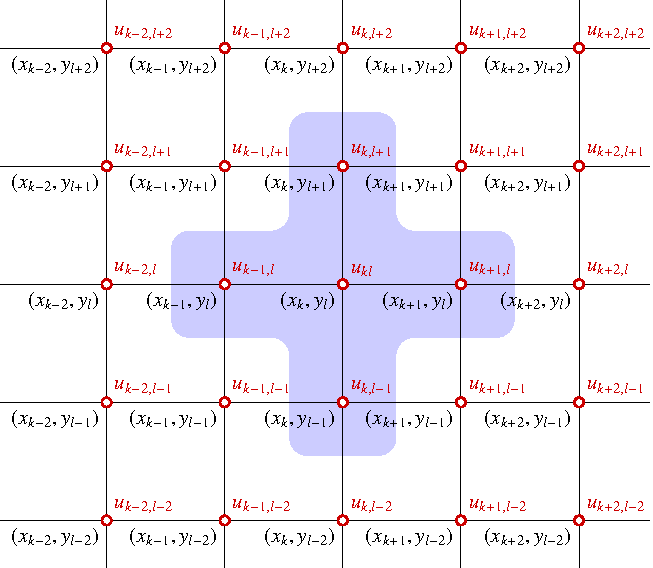
\includegraphics{chapters/090-pdenumerik/images/2d.pdf}
\caption{Diskretisation mit finiten Differenzen in zwei Dimension.
Für jeden Gitterpunkt wird einen Variable ({\color{darkred}rot}) benötigt.
Für die Berechnung einer Approximation des Laplace-Operators an der
Stelle $(x_k,y_l)$ sind die Variablen im blauen Kreuz notwendig.
\label{buch:pdenumerik:fdm:fig:2d}}
\end{figure}
%
Für ein Gitter von Punkten $(x_k,y_l) = (kh,lh)$ mit Schrittweite $h$
wie in Abbildung~\ref{buch:pdenumerik:fdm:fig:2d}
schreiben wir $u_{kl}=u(x_k,y_l)$ für die Werte der Lösungsfunktion.
Die Ableitungen können dann wieder durch die Differenzenquotienten
\begin{align*}
\frac{\partial u}{\partial x}(x_k,y_k)
&\approx
\frac{u_{k+1,l}-u_{kl}}{h}
&
\frac{\partial u}{\partial y}(x_k,y_k)
&\approx
\frac{u_{k,l+1}-u_{kl}}{h}
\\
\frac{\partial^2 u}{\partial x^2}(x_k,y_k)
&=
\frac{u_{k+1,l}-2u_{kl}+u_{k-1,l}}{h^2}
&
\frac{\partial^2 u}{\partial x^2}(x_k,y_k)
&=
\frac{u_{k,l+1}-2u_{kl}+u_{k,l-1}}{h^2}
\end{align*}
approximieren.
Die Differentialgleichung wird dann durch die lineare Gleichung
\[
\Delta u(x_k,y_k)
\approx
\frac{1}{h^2}
\bigl(
u_{k+1,l}+u_{k-1,l}+u_{k,l+1}+u_{k,l-1} - 4 u_{kl}
\bigr)
=
f_{kl} = f(x_k,y_l)
\]
ersetzt.

